\section{Experimental Results}
\label{sec:result}

This section presents experiment results and answer the RQs by
studying the results quantatively and qualitatively.

\InputWithSpace{tables/manual-study-table}
\InputWithSpace{tables/test-results-table}
\subsection{RQ1: \tool Sentiment Label Consistency}
Table~\ref{table:ManualStudy} shows results of our manual study. The
first column represents type of test case. The number of test cases
used for the study is represented in second column. The label
consistency score defined in equation~\ref{metric:srel} is shown in
column 3.

We observe that \emph{\tool generates test cases that consistently
  label their sentiment correctly.}  Column 3 shows that the label
consistency scores are 0.83 and 0.84 for the seed and expanded
sentences, respectively. We can observe that the scores are not same
as maximum scores meaning that there are inconsistency on labels
between \tool and subjects. The cuases of inconsistency in the scores
are two following: First, complicated sentence leads subjects to
misunderstand its meaning. Second, phrase in a sentence introduces its
multiple interpretations to understand its sentiment. For example, the
word ``easy'' could be interpreted as both compliment and back-handed
insult.  This means that \tool generates test oracles consistent with
human understanding most of the time. It is observed that there is
little difference of the scores between the seed and expanded
sentences. This implies that the syntax-based sentence expansion in
\tool preserves the sentiment as its seed.
%% \sw{What are
%%   the causes of inconsistency? Looks like the main source of
%%   inconsistency comes from seed generation? Any insights on how it
%%   happened (e.g., issue with original labels, search rules, or
%%   templates?}

\subsection{RQ2: Correctness of Linguistic Capability Categorization}
The \lc relevancy score defined in~\ref{metric:lcrel} is shown in
column 4 of Table \ref{table:ManualStudy}. The result shows that
\emph{\tool generates test cases that are correctly categorized to the
  corresponding linguistic capabilities most of the time.}  The \lc
relevancy scores for the seed and expanded sentences are both 0.9,
achieving high order of agreement with human assessment. The fact that
the expanded sentences generated by \tool also have same level of \lc
relevancy as the seed sentences shows that the syntax-based sentence
expansion retains the linguistic capabilities.
%% \sw{Source of incorrect
%% categorization of linguistic capabilities?}


\subsection{RQ3: Test Suite Diversity}

We first show evaluation results of three \sa models via
table~\ref{table:TestResult}. In the table, first column lists
linguistic capability for \sa task, and Columns 2-3 show the number of
seed and expanded test cases respectively. Columns 4-5 show the
failure rate in percentage by evaluating the \sa models on the seed
and expanded test cases respectively. Column 6 shows the number of
expanded test cases failed, but their seed test cases passed.  From
the table, we can observe that LC3 has no expanded sentences from its
seeds. It means that the 50 seeds selected in this experiment does not
provide any validated expansions. It is because the randomness of
selection of 50 seeds determines the number of validated
expansions. we expect that more selection of seeds increases the
probability of availability of their expansion. In addition, LC1 and
LC5 obtains 19 and 26 seeds respectively. It represents that \tool
finds and generates their seeds lower than the target number of seeds,
which is 50 in this experiment. In this case, use of larger search
dataset increases the amount of seeds for the \lcs. From the table, it
is found that all three models achieves better performance on LC9 and
LC2 while they obatains high failure rates on other \lcs. Finally, we
find that there are number of a number of failed expanded test cases
succeeded before the expansion (pass on seed, but fail on its expanded
test cases). This shows that phase of syntax-based sentence expansion
in \tool captures failure-inducing expansion given a seed. It finally
shows usefulness of \tool since the different test results between
seed and expanded cases provide accurate guidance for debugging model.


\begin{figure}
    \centering
    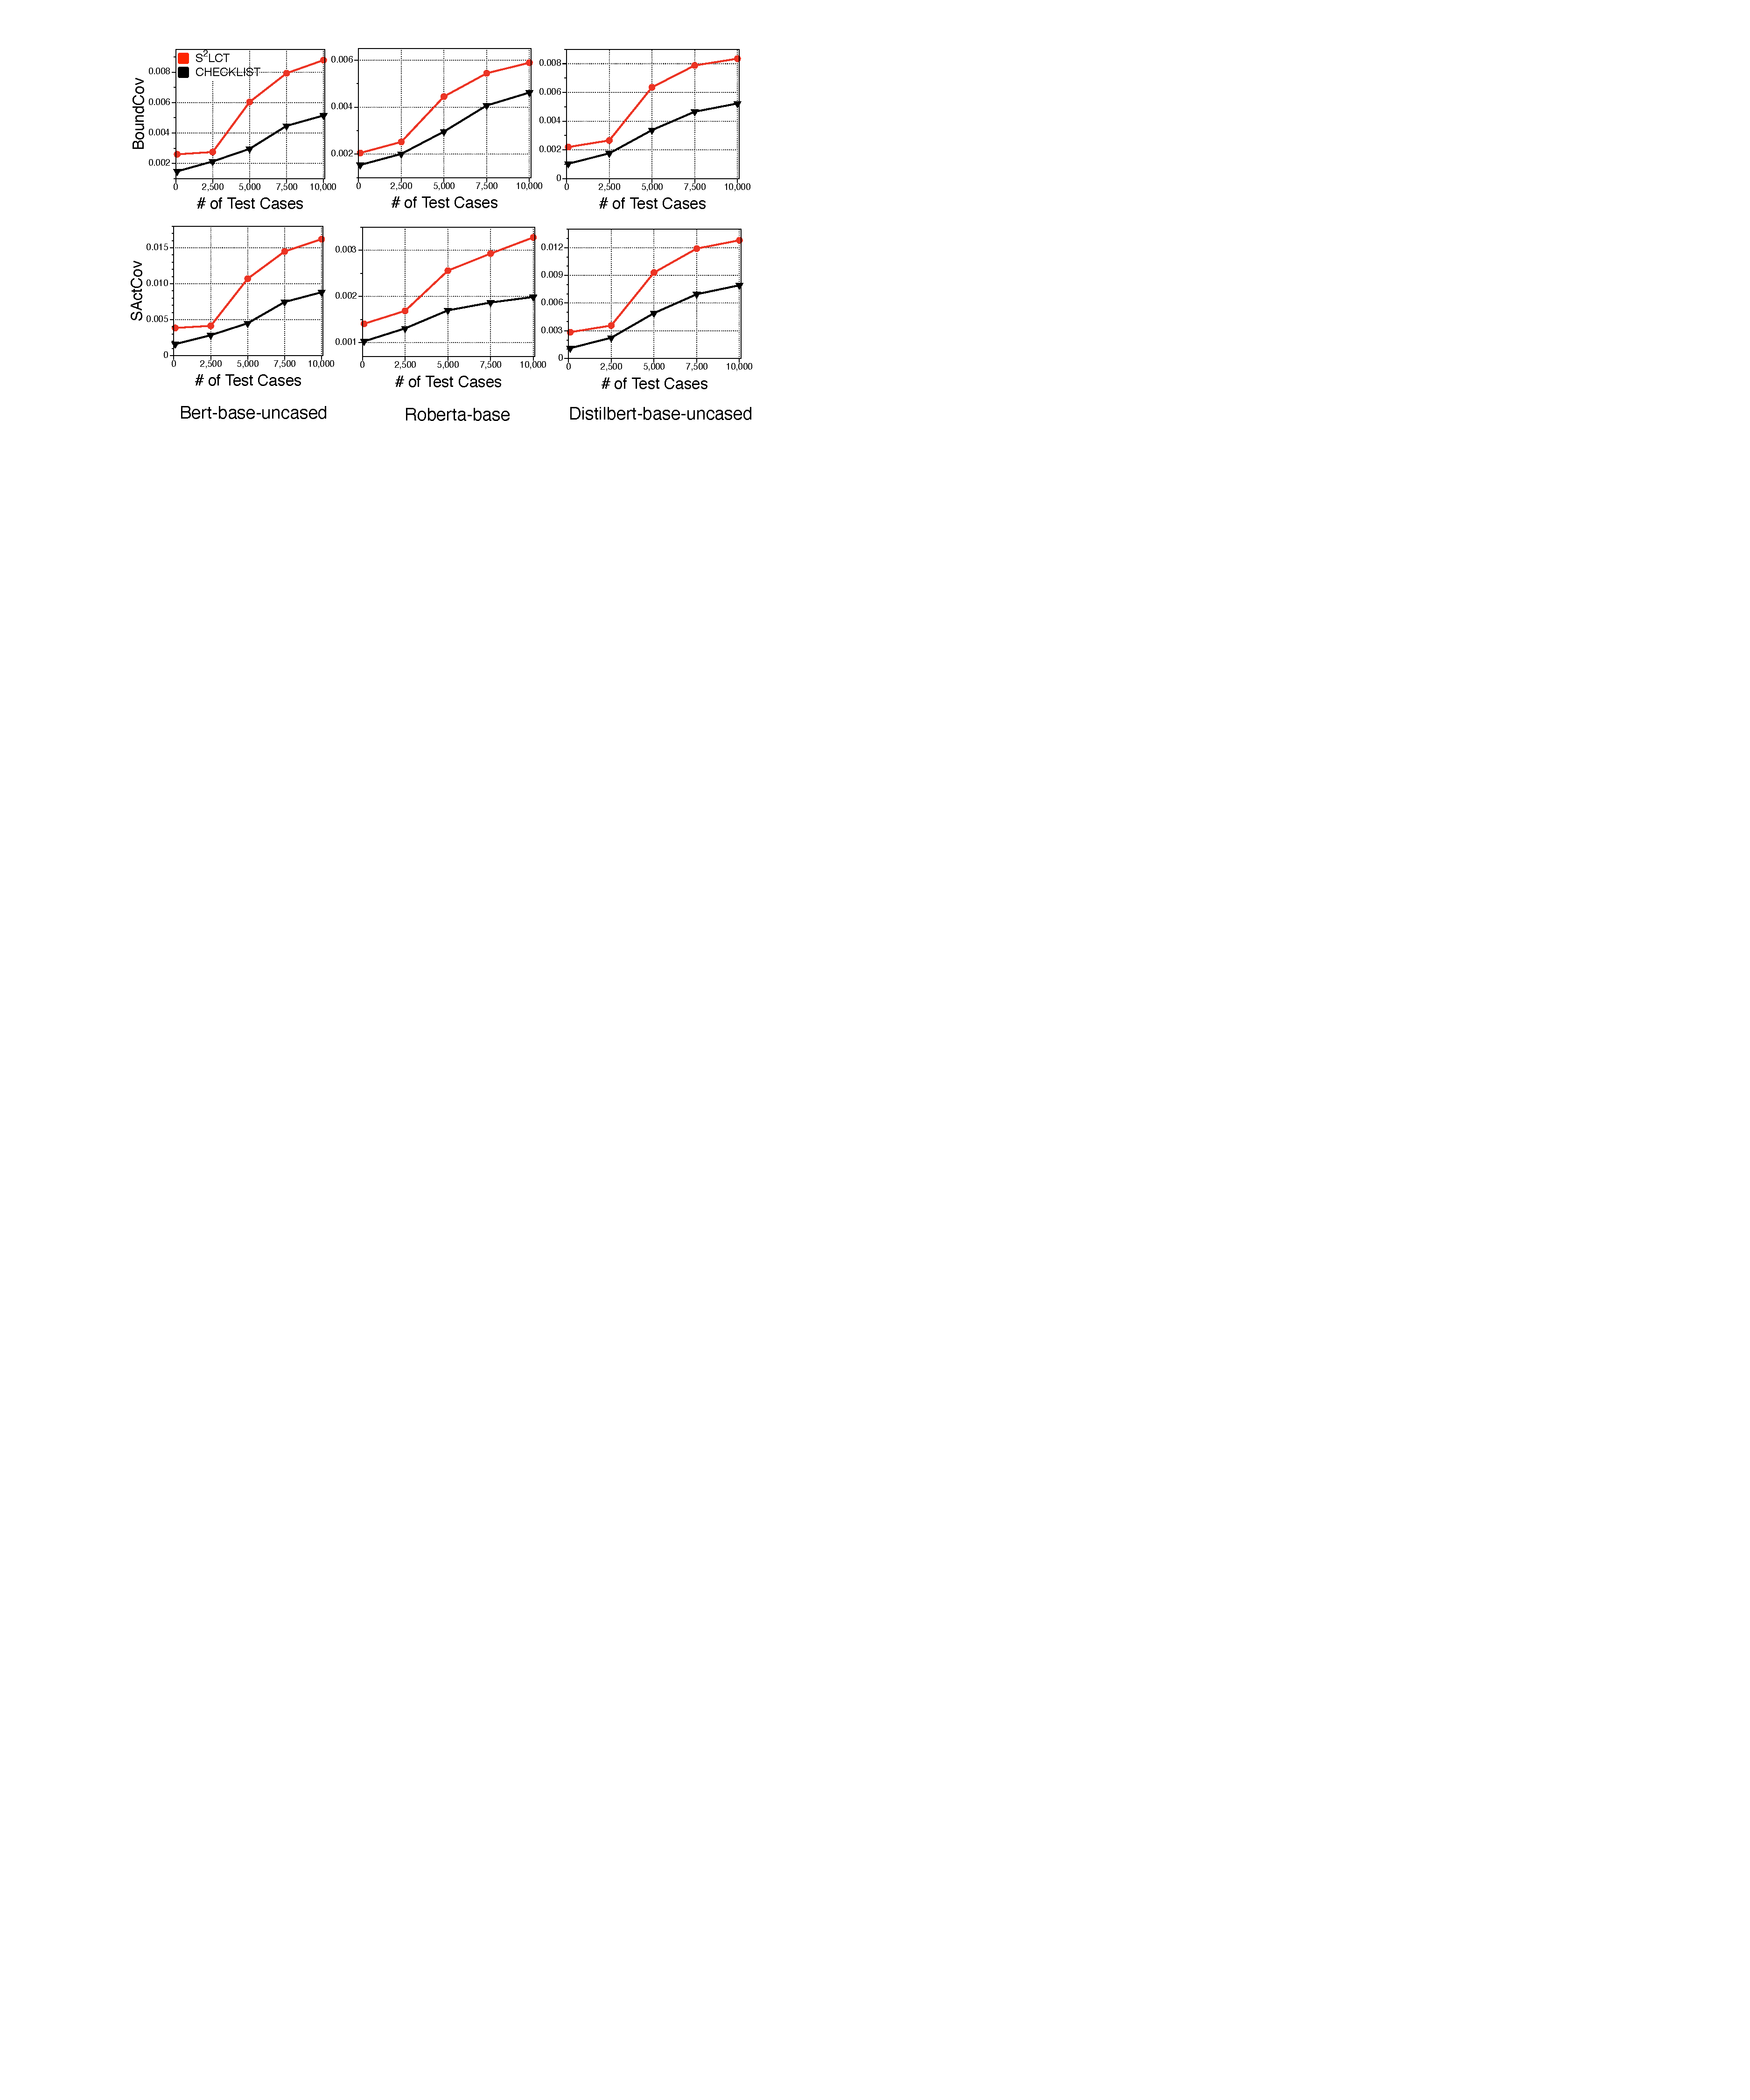
\includegraphics[width=0.5\textwidth]{figs/coverage.pdf}
    \vspace{-4mm}
    \caption{Coverage results of \tool and \Cklst test cases.}
    \label{fig:coverage}
\end{figure}

Next, Figure \ref{fig:coverage} shows the coverage results of \tool and \Cklst test cases. The red line represents \tool coverage and the black line represents \Cklst coverage. Each column in Figure \ref{fig:coverage} represents the results for one NLP model. The first row is the \textit{BoundCov} results and the second row is the \textit{SActCov} results.

We made three observations.
First, for \emph{all} experimental settings (i.e., NLP model and coverage metric), \tool achieves higher coverage than \Cklst. Recall that a higher coverage implies the test cases are more diverse and do not have a similar statistical distribution to the model training data. As a result, a test suite with greater coverage complements the model training data distribution (\ie holdout testing data) better.
For example, for the first NLP model under test, \tool can achieve a higher coverage than \Cklst with only half the number of test cases.
This result confirms that \tool can generate more diverse test cases to complement the holdout dataset for testing NLP models.

Second, as the number of test cases increases, the test suite can achieve better coverage. Such observation is intuitive. However, generating a more extensive test suite is not easy, particularly  for \Cklst, which is a manually template-based approach.

Third, for each NLP model, there is no fixed relationship between \textit{BoundCov} and \textit{SActCov}. In other words, while a test suite may produce higher \textit{BoundCov} for some models, the same test suite may get higher \textit{SActCov} for other NLP models.
Recall that \textit{BoundCov} measures both the upper and lower corner neurons and \textit{SActCov} measures only the upper corner neurons. 
Such observation implies that the upper and lower corner neurons are distributed unevenly, and measuring only one of them is not enough.

\subsection{RQ4: Use \tool for Debugging}
